\begin{figure}[!ht]
    \centering
        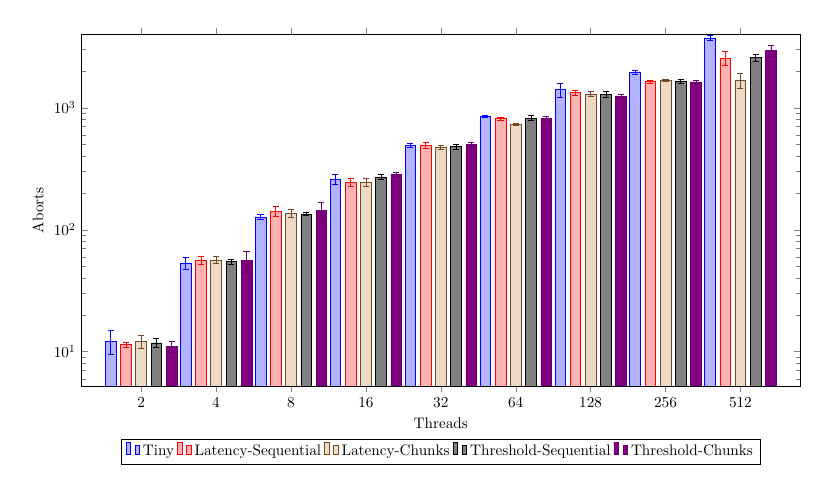
\begin{tikzpicture}[scale=0.55, baseline]
        \begin{axis}[
            ymode=log,
            width=1.5 \linewidth,
            height=0.8 \linewidth,
            %media de tempo intruder
            ybar=3pt,
            %enlargelimits=0.10,
            legend style={at={(0.5,-0.15)}, anchor=north, legend columns=-1},
            ylabel=Aborts,
            xlabel=Threads,
            symbolic x coords={1, 2, 4, 8, 16, 32, 64, 128, 256, 512},
            xtick=data,
            ymin=0,
            ymax=4000,
            bar width=7pt,
            % nodes near coords,
            nodes near coords align={vertical},
        ]
        \addplot+[error bars,y dir=both, y explicit] coordinates {
            (1,0.0)+-(1,0.0) (2,12.2)+-(2,2.63) (4,53.2)+-(4,5.94) (8,127.2)+-(8,6.14) (16,258.0)+-(16,24.04) (32,490.2)+-(32,16.41) (64,847.0)+-(64,12.39) (128,1413.4)+-(128,186.85) (256,1959.6)+-(256,67.08) (512,3727.2)+-(512,167.11) 
        };
        \addplot+[error bars,y dir=both, y explicit] coordinates {
            (1,0.0)+-(1,0.0) (2,11.4)+-(2,0.48) (4,56.0)+-(4,4.09) (8,142.0)+-(8,12.85) (16,245.8)+-(16,19.87) (32,491.2)+-(32,25.11) (64,811.8)+-(64,28.18) (128,1334.2)+-(128,63.09) (256,1633.4)+-(256,41.57) (512,2556.6)+-(512,340.72)
        };
        \addplot+[error bars,y dir=both, y explicit] coordinates {
             (1,0.0)+-(1,0.0) (2,12.2)+-(2,1.46) (4,56.4)+-(4,3.61) (8,136.4)+-(8,10.30) (16,245.4)+-(16,19.39) (32,473.2)+-(32,16.47) (64,734.8)+-(64,11.12) (128,1298.4)+-(128,60.09) (256,1677.2)+-(256,35.19) (512,1686.8)+-(512,244.04)
        };
        \addplot+[error bars,y dir=both, y explicit] coordinates {
            (1,0.0)+-(1,0.0) (2,11.8)+-(2,0.97) (4,54.8)+-(4,2.78) (8,134.8)+-(8,4.39) (16,271.2)+-(16,11.35) (32,482.8)+-(32,22.57) (64,822.0)+-(64,36.78) (128,1291.2)+-(128,74.59) (256,1657.8)+-(256,58.13) (512,2571.6)+-(512,174.36)
        };
        \addplot+[error bars,y dir=both, y explicit] coordinates {
            (1,0.0)+-(1,0.0) (2,11.0)+-(2,1.2) (4,55.72)+-(4,10.82) (8,143.2)+-(8,25.75) (16,286.0)+-(16,10.86) (32,496.6)+-(32,19.73) (64,812.0)+-(64,38.57) (128,1238.6)+-(128,53.69) (256,1629.6)+-(256,55.64) (512,2933.4)+-(512,289.46)
        };
        \legend {Tiny, Latency-Sequential, Latency-Chunks, Threshold-Sequential, Threshold-Chunks}
        \end{axis}
        \end{tikzpicture}
    \caption{Aborts do benchmark Labyrinth variando o número de \emph{threads}.}
    \label{labyrinth_abort}

\end{figure}